\documentclass{beamer}

\usetheme{Boadilla}
% \usecolortheme{beaver} % --- We are replacing this with our own theme below ---

\usepackage{amsmath}
\usepackage{amssymb}
\usepackage{graphicx}
\usepackage{physics}
\usepackage{mathtools}
\usepackage{siunitx}
\usepackage{tikz}
\usetikzlibrary{positioning, shapes.geometric, arrows.meta}
\usepackage{booktabs}
\usepackage{lmodern}
\usepackage{setspace}
\onehalfspacing
\usepackage[bottom]{footmisc}

% --- CUSTOM COLOR THEME SETUP ---

% 1. Define your new colors using Hex codes
\definecolor{ULBBlue}{HTML}{0D47A1}
\definecolor{ULBTeal}{HTML}{4DB6AC}
\definecolor{VUBOrange}{HTML}{E87722}
\definecolor{AlertColor}{HTML}{D32F2F}
\definecolor{LightGray}{HTML}{F5F5F5}


% 2. Apply these colors to Beamer's elements
\setbeamercolor{palette primary}{bg=ULBBlue, fg=white}
\setbeamercolor{palette secondary}{bg=VUBOrange, fg=white}
\setbeamercolor{palette tertiary}{bg=ULBBlue, fg=white}
\setbeamercolor{palette quaternary}{bg=VUBOrange, fg=white}

\setbeamercolor{structure}{fg=ULBBlue} % This is a key color for many elements
\setbeamercolor{titlelike}{bg=ULBBlue, fg=white}
\setbeamercolor{frametitle}{bg=ULBBlue, fg=white}
\setbeamercolor{title}{use=structure,fg=white,bg=structure.fg}

\setbeamercolor{normal text}{fg=black, bg=white}
\setbeamercolor{block title}{use=structure,fg=white,bg=structure.fg}
\setbeamercolor{block body}{bg=LightGray}
\setbeamercolor{alerted text}{fg=AlertColor}

% --- END OF CUSTOM COLOR THEME ---

% --- Command to automatically create a title slide for each section ---
\AtBeginSection[]{
	\begin{frame}
		\vfill
		\centering
		\begin{beamercolorbox}[sep=8pt,center,shadow=true,rounded=true]{title}
			\usebeamerfont{title}\insertsectionhead\par%
		\end{beamercolorbox}
		\vfill
	\end{frame}
}
% --- END of command ---


\title[Shadowing, Cell Coverage, and Link Budgets]{Question 3: Shadowing, Cell Coverage, and Link Budgets}
\subtitle{Statistical Model and Practical Implications}
\author{Cédric Sipakam}
\institute{ULB | VUB \\
	\vspace{1.5em}
	ELEC-H415: Communication Channels}
\date{2025}


\setbeamertemplate{footline}
{
	\leavevmode%
	\hbox{%
		\begin{beamercolorbox}[wd=.5\paperwidth,ht=2.25ex,dp=1ex,left]{author in head/foot}%
			\hspace*{2ex}\usebeamerfont{title in head/foot}\insertshorttitle%
		\end{beamercolorbox}%
		\begin{beamercolorbox}[wd=.5\paperwidth,ht=2.25ex,dp=1ex,right]{title in head/foot}%
			\usebeamerfont{page number in head/foot}\insertframenumber{} / \inserttotalframenumber\hspace*{2ex}%
		\end{beamercolorbox}%
	}%
	\vskip0pt%
}



\begin{document}
	\begin{frame}
		\begin{figure}
			\centering
			
\includegraphics[width=0.7\linewidth]{pictures/logos}
		\end{figure}
		\titlepage
	\end{frame}
	
	\begin{frame}{Outline}
		\tableofcontents
	\end{frame}
	
	\section{The Shadowing Statistical Model}
	
	\begin{frame}{Components of Received Power Variation}
		\begin{itemize}
			\item The received power $P_{RX}$ is not constant but varies due to several effects.
			\item It is modeled as the combination of three main components:
			\begin{enumerate}
				\item \textbf{Path Loss}: The average power decay with distance, $\ll P_{RX} \gg$.
				\item \textbf{Shadowing (or Slow Fading)}: Large-scale variations around the path loss mean, caused by obstacles like buildings and hills, $<P_{RX}>$.
				\item \textbf{Small-Scale Fading (or Fast Fading)}: Rapid fluctuations due to multipath interference, $P_{RX}$.
			\end{enumerate}
		\end{itemize}
	\end{frame}
	
	\begin{frame}{Components of Received Power Variation}
		\begin{figure}
			\centering
			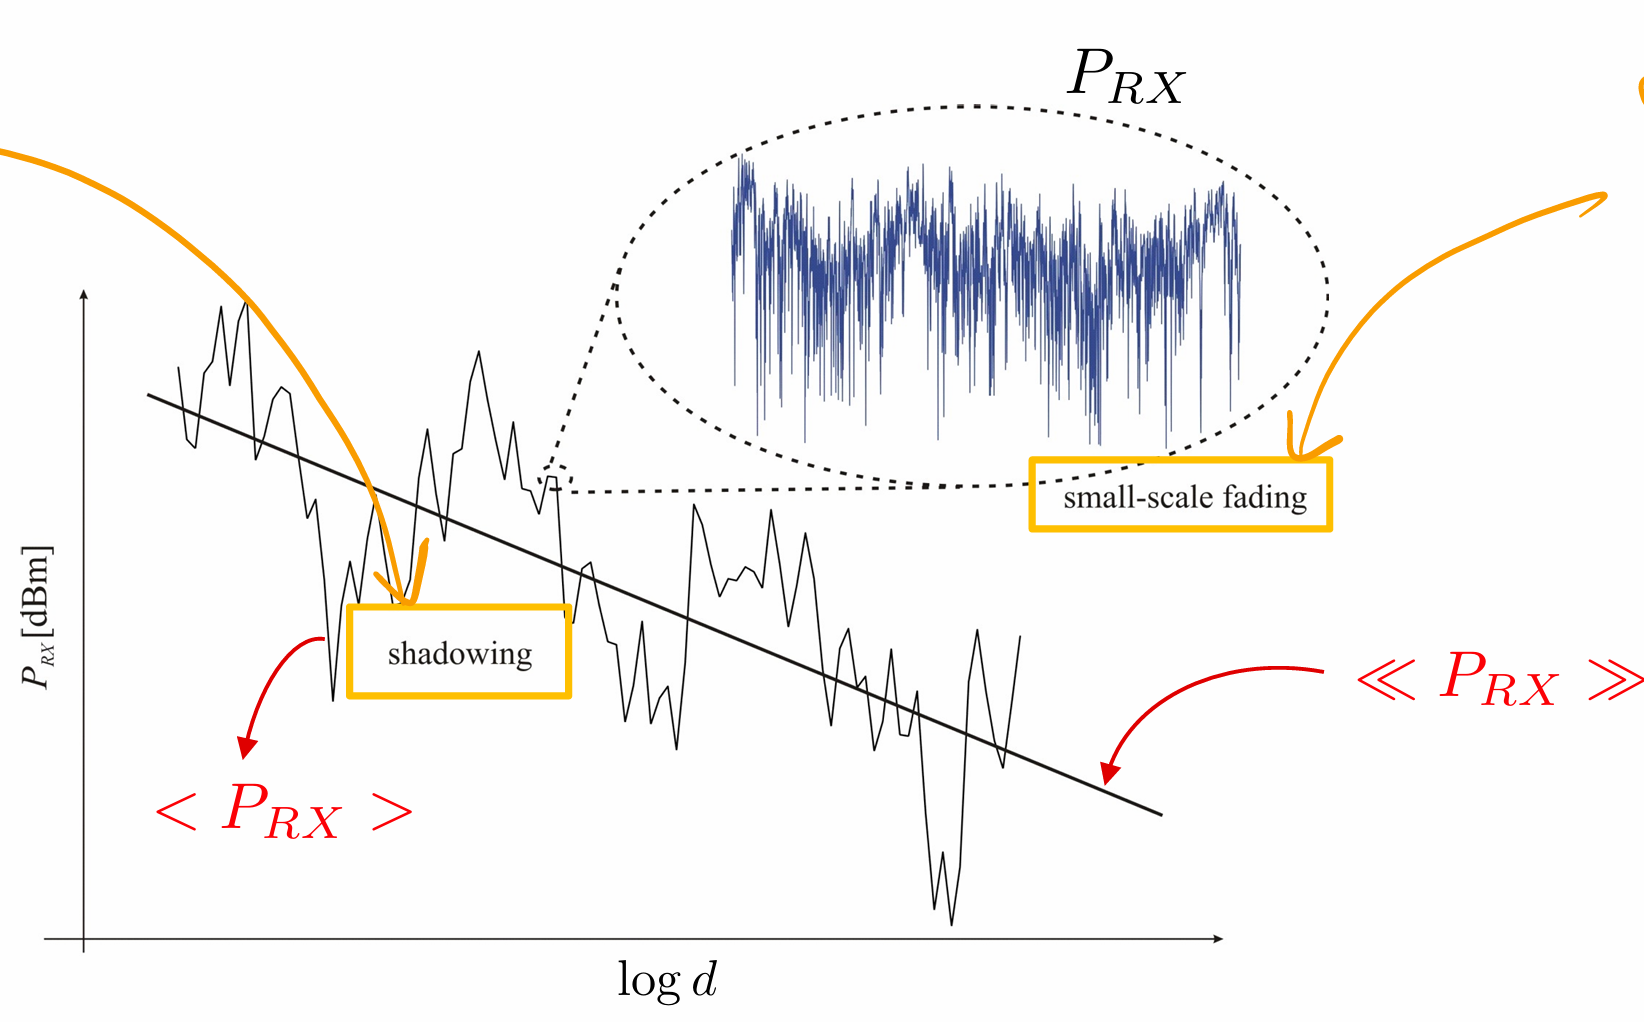
\includegraphics[width=0.8\linewidth]{"pictures/power-components.png"}
			\caption{Illustration of path loss, shadowing, and small-scale fading.}
		\end{figure}
	\end{frame}
	
	\begin{frame}{Defining the Statistical Model}
		\begin{itemize}
			\item Shadowing describes the random variations of the locally averaged received power, $<P_{RX}>$, around the mean power, $\ll P_{RX} \gg$, predicted by a path loss model.
			\item Experimental data shows that when the received power is expressed in decibels (dB or dBm), the variations due to shadowing follow a \textbf{Normal (Gaussian) distribution}.
			\item This means the power in linear units (Watts) follows a \textbf{log-normal distribution}.
		\end{itemize}
	\end{frame}
	
	\begin{frame}{Mathematical Formulation}
		\begin{itemize}
			\item The locally averaged received power in dBm is modeled as:
			\[
			<P_{RX}>(d)[\text{dBm}] = \ll P_{RX} \gg[\text{dBm}] - L_{\sigma_L}
			\]
			\item Where:
			\begin{itemize}
				\item $\ll P_{RX} \gg[\text{dBm}]$ is the mean power at distance $d$ from the path loss model.
				\item $L_{\sigma_L}$ is a zero-mean Gaussian random variable with standard deviation $\sigma_L$.
			\end{itemize}
			\item The parameter $\sigma_L$, known as the \textbf{shadowing variability} or standard deviation, is determined empirically and typically ranges from \SI{4}{\decibel} to \SI{10}{\decibel} depending on the environment.
		\end{itemize}
	\end{frame}
	
	\begin{frame}{Mathematical Formulation}
		\begin{figure}
			\centering
			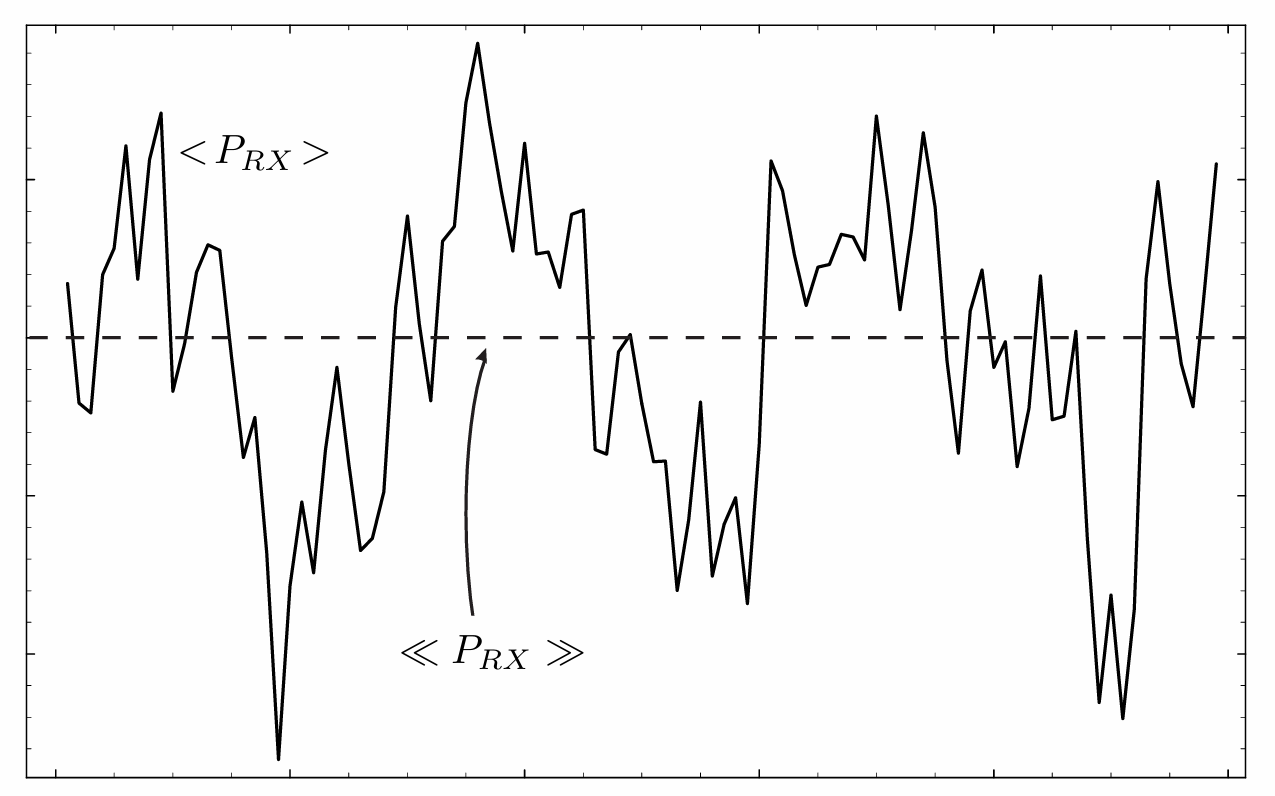
\includegraphics[width=0.7\linewidth]{"pictures/shadowing-variations.png"}
			\caption{Example of shadowing variations around the mean predicted by path loss.}
		\end{figure}
	\end{frame}
	
	\section{Impact of Shadowing on Cell Coverage}
	
	\begin{frame}{The Challenge of Defining Cell Radius}
		\begin{itemize}
			\item A cell's boundary is defined by the distance at which the received power drops to the receiver's minimum required level, known as its \textbf{sensitivity}.
			\item If we ignore shadowing and define the cell radius $R$ as the distance where the \textit{mean} received power equals the sensitivity, we encounter a problem.
			\[ \ll P_{RX}(R) \gg = \text{sensitivity} \]
		
		\end{itemize}
		
	\end{frame}
	
	\begin{frame}{The Challenge of Defining Cell Radius}
		\begin{itemize}
		
			\item Since shadowing is a zero-mean Gaussian process, this definition implies that at the cell edge, the actual received power $<P_{RX}>$ will be below the sensitivity threshold for 50\% of the locations.
		\end{itemize}
		\begin{alertblock}{Conclusion}
			A 50\% service reliability at the cell edge is unacceptable for most communication systems.
		\end{alertblock}
	\end{frame}
	
	\begin{frame}{The Challenge of Defining Cell Radius}
		\begin{figure}
			\centering
			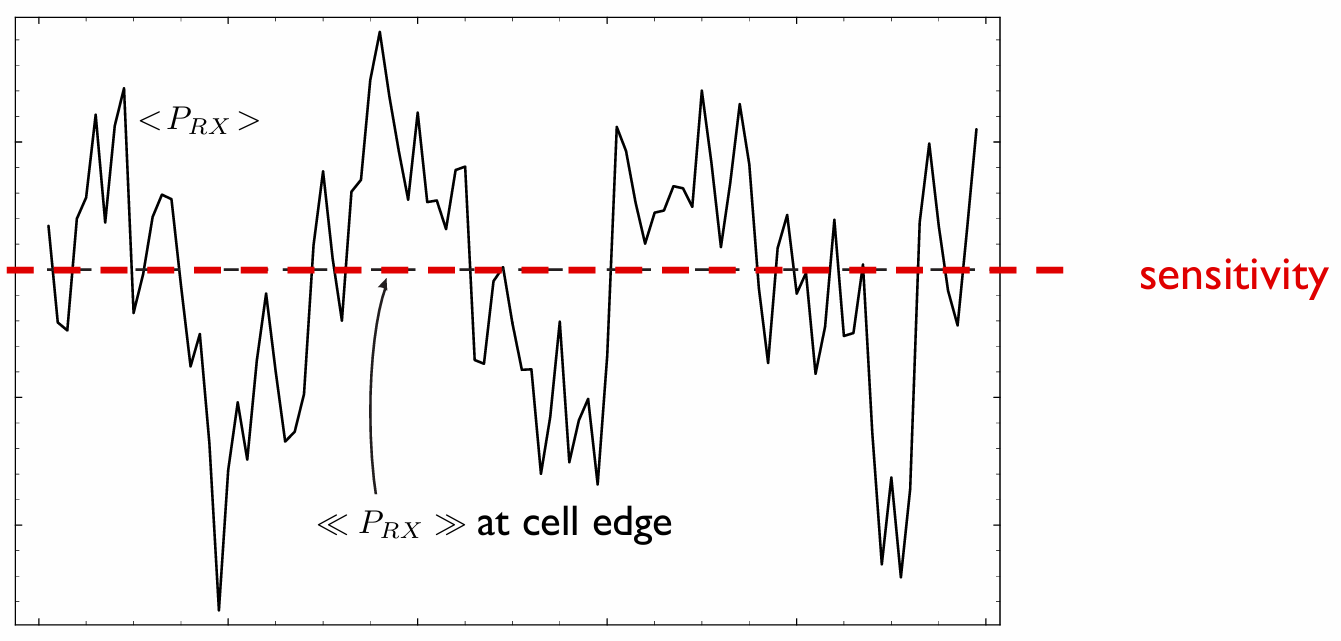
\includegraphics[width=0.9\linewidth]{"pictures/50-percent-problem.png"}
			\caption{At the cell edge (R), 50\% of locations fall below the sensitivity threshold.}
		\end{figure}
	\end{frame}
	
	\begin{frame}{The Challenge of Defining Cell Radius}
		\begin{figure}
			\centering
			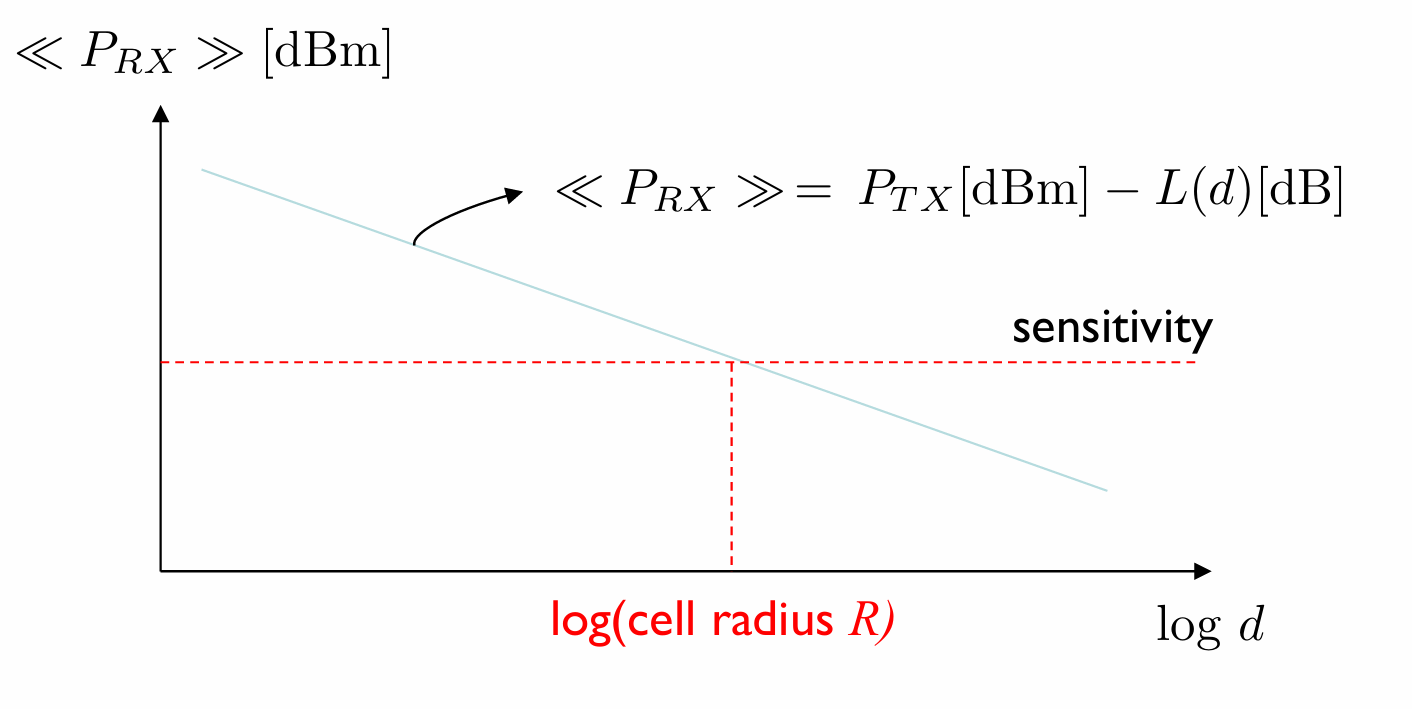
\includegraphics[width=0.9\linewidth]{"pictures/50-percent-problem-2.png"}
			\caption{At the cell edge (R), 50\% of locations fall below the sensitivity threshold.}
		\end{figure}
	\end{frame}
	
	\begin{frame}{The Solution: The Fade Margin}
		\begin{itemize}
			\item To ensure a higher reliability, we must design the system so that the mean received power at the cell edge is \textit{greater} than the sensitivity.
			\item This buffer is called the \textbf{Fade Margin}, $M$.
			\item The cell radius $R$ is now defined by the condition:
			\[ \ll P_{RX}(R) \gg[\text{dBm}] = \text{sensitivity} + M \]
			\item This is equivalent to reducing the maximum allowed path loss:
			\[ L(R) = L_{max} - M \]
		\end{itemize}
	\end{frame}
	
	\begin{frame}{The Solution: The Fade Margin}
		\begin{figure}
			\centering
			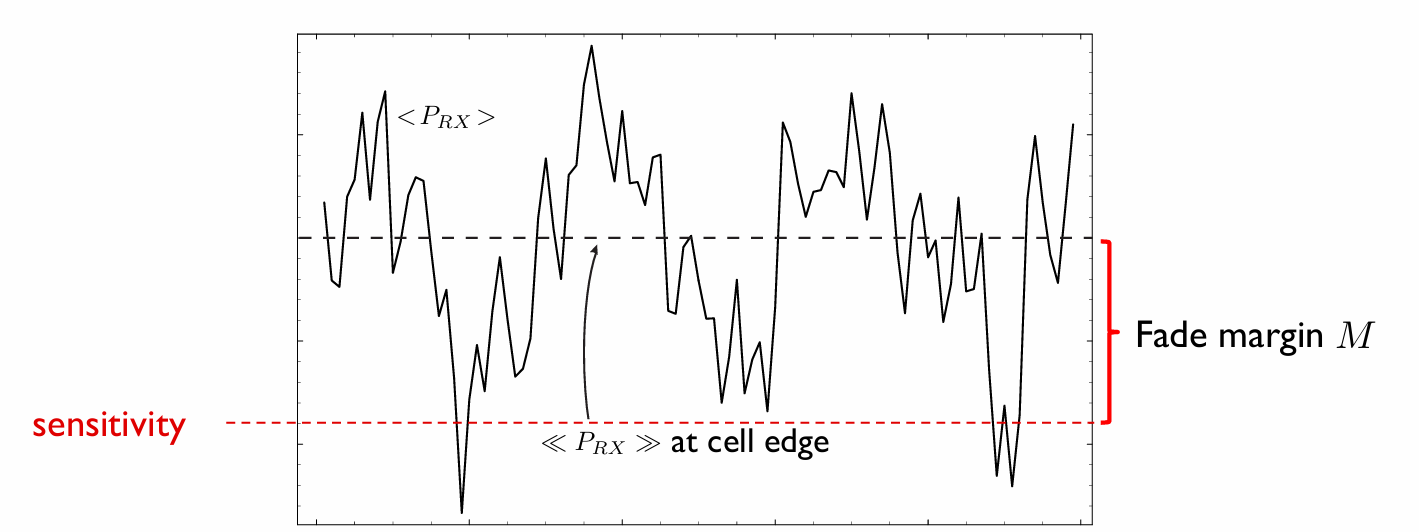
\includegraphics[width=0.9\linewidth]{"pictures/fade-margin-concept.png"}
			\caption{Introducing a fade margin $M$ increases the mean power at the new, smaller cell edge, improving reliability.}
		\end{figure}
	\end{frame}
	
	\begin{frame}{The Solution: The Fade Margin}
		\begin{figure}
			\centering
			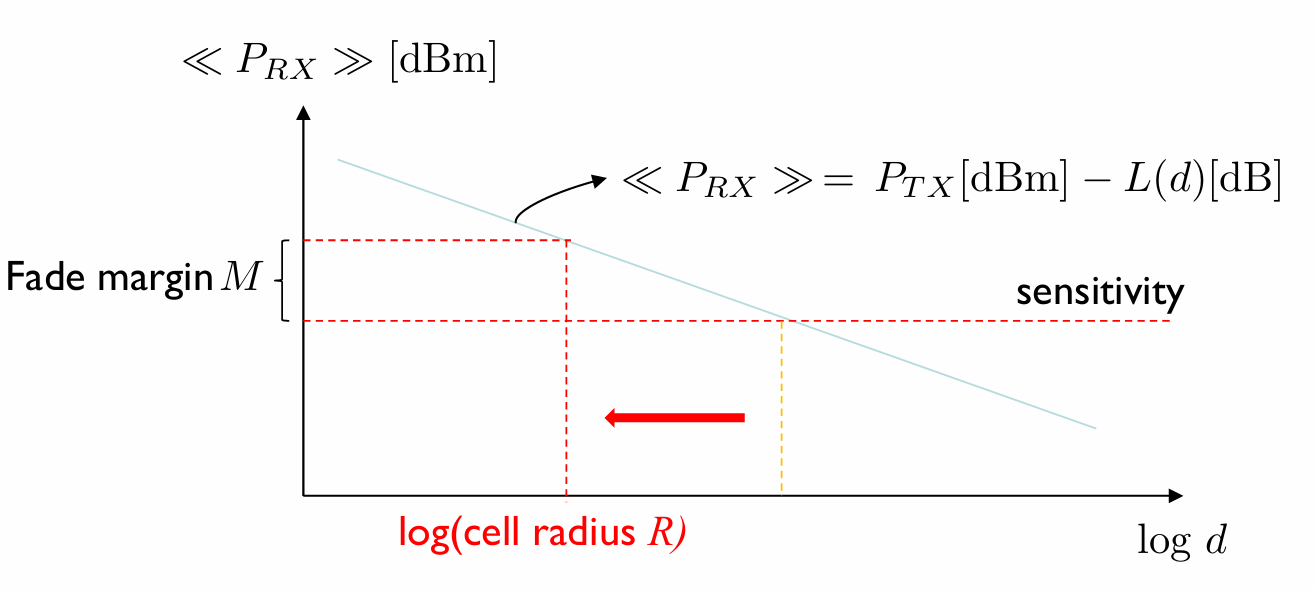
\includegraphics[width=0.9\linewidth]{"pictures/fade-margin-concept-2.png"}
			\caption{Introducing a fade margin $M$ increases the mean power at the new, smaller cell edge, improving reliability.}
		\end{figure}
	\end{frame}
	
	\begin{frame}{Demonstration: Overall Cell Coverage (1/3)}
		\begin{itemize}
			\item We want to find the overall service probability, $F_u$, within a cell of radius $R$. This is the probability that the received power is above the sensitivity.
			\item The probability of an outage (connection failure) at a distance $r$ is the probability that the total path loss exceeds the maximum allowed loss, $L_{max}$:
			\[ P_{\text{outage}}(r) = \text{Pr}[L(r) + L_{\sigma_L} > L_{max}] = \text{Pr}[L_{\sigma_L} > L_{max} - L(r)] \]
			\item Let $l(r) = L_{max} - L(r)$. The outage probability is then:
			\[ P_{\text{outage}}(r) = \text{Pr}[L_{\sigma_L} > l(r)] = \frac{1}{2}\text{erfc}\left(\frac{l(r)}{\sigma_L\sqrt{2}}\right) \]
		\end{itemize}
	\end{frame}
	
	\begin{frame}{Demonstration: Overall Cell Coverage (2/3)}
		\begin{itemize}
			\item To find the average outage probability over the entire cell, we integrate over the cell area:
			\[ \bar{P}_{\text{outage}} = \frac{1}{\pi R^2} \int_0^R P_{\text{outage}}(r) \, 2\pi r \, dr \]
			\item The overall coverage probability is $F_u = 1 - \bar{P}_{\text{outage}}$:
			\[ F_u = 1 - \frac{2}{R^2} \int_0^R \frac{1}{2}\text{erfc}\left(\frac{l(r)}{\sigma_L\sqrt{2}}\right) r \, dr \]
			\item We use the canonical path loss model: $L(r) = L(R) + 10n \log_{10}(r/R)$.
			\item Therefore, $l(r) = L_{max} - L(R) - 10n \log_{10}(r/R) = M - 10n \log_{10}(r/R)$.
		\end{itemize}
	\end{frame}
	
	\begin{frame}{Demonstration: Overall Cell Coverage (3/3)}
		\begin{itemize}
			\item The integral becomes:
			\[ F_u = 1 - \frac{1}{R^2} \int_0^R \text{erfc}\left( \frac{M - 10n \log_{10}(r/R)}{\sigma_L\sqrt{2}} \right) r \, dr \]
			\item Let $a = \frac{M}{\sigma_L\sqrt{2}}$ and $b = \frac{10n \log_{10}(e)}{\sigma_L\sqrt{2}}$. The argument of erfc is $(a - b \ln(r/R))$.
			
		\end{itemize}
		
	\end{frame}
	
	\begin{frame}{Demonstration: Overall Cell Coverage (3/3)}
		\begin{itemize}
			
			\item Solving this integral yields the final result for cell coverage probability:
			\[ F_u = 1 - \frac{1}{2}\text{erfc}(a) + \frac{1}{2}e^{2a/b + 1/b^2} \text{erfc}\left(a + \frac{1}{b}\right) \]
		\end{itemize}
		\begin{block}{Conclusion}
			The overall cell coverage is a direct function of the chosen fade margin ($M$), the environment's path loss exponent ($n$), and its shadowing variability ($\sigma_L$).
		\end{block}
	\end{frame}
	
	\begin{frame}{Demonstration: Overall Cell Coverage}
		\begin{figure}
			\centering
			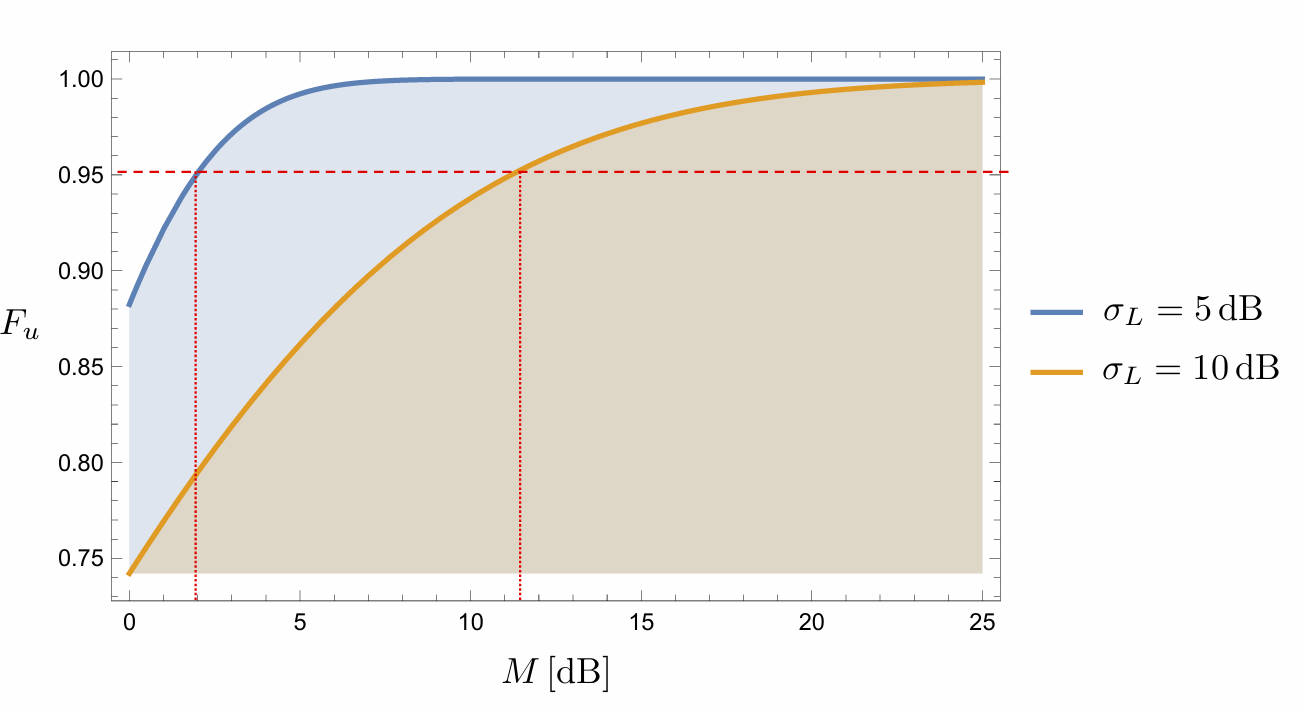
\includegraphics[width=0.9\linewidth]{"pictures/fu-vs-margin.png"}
			\caption{Cell coverage probability ($F_u$) vs. Fade Margin ($M$) for different shadowing variabilities ($\sigma_L$).}
		\end{figure}
	\end{frame}
	
	\section{Shadowing in Link Budgets}
	
	\begin{frame}{The Role of a Link Budget}
		\begin{itemize}
			\item A link budget is a systematic accounting of all gains and losses in a communication system.
			\item Its primary goal is to calculate the maximum allowed path loss ($L_{max}$) that the system can tolerate while still meeting a target performance metric (e.g., a minimum Signal-to-Noise Ratio, SNR).
			\item Shadowing is a critical "loss" that must be accounted for to ensure reliable communication.
		\end{itemize}
	\end{frame}
	
	\begin{frame}{Example: Cellular Downlink Budget}
		\begin{itemize}
			\item Let's analyze how shadowing is incorporated into a typical link budget.
			\item The goal is to find the maximum path loss. We start with the transmitter's power and subtract all losses and required margins until we reach the receiver's sensitivity.
			\item The \textbf{Shadowing Margin} (or Fade Margin) is explicitly included as one of these required margins.
		\end{itemize}
	\end{frame}
	
	\begin{frame}{Example: Cellular Downlink Budget}
		\centering
		\resizebox{0.85\textwidth}{!}{%
			\begin{tabular}{lllr}
				\toprule
				\textbf{Parameter} & \textbf{Symbol} & \textbf{Calculation} & \textbf{Value} \\
				\midrule
				\multicolumn{1}{c}{\textbf{Transmitter Side (Gains)}} \\
				TX Power & $P_{TX}$ & Given & \SI{43}{dBm} \\
				TX Antenna Gain & $G_{TX}$ & Given & \SI{15}{dBi} \\
				\textbf{Effective Isotropic Radiated Power} & \textbf{EIRP} & $P_{TX} + G_{TX}$ & \textbf{\SI{58}{dBm}} \\
				\midrule
				\multicolumn{1}{c}{\textbf{Receiver Side (Requirements)}} \\
				Thermal Noise Power ($T_0=\SI{290}{K}, B=\SI{10}{MHz}$) & & $10\log_{10}(kT_0B/\SI{1}{mW})$ & \SI{-104}{dBm} \\
				RX Noise Figure & $F_{dB}$ & Given & \SI{7}{dB} \\
				Receiver Noise Floor & $N$ & & \SI{-97}{dBm} \\
				Target Signal-to-Noise Ratio & SNR & Required for service & \SI{1}{dB} \\
				\textbf{Receiver Sensitivity} & & $N + \text{SNR}$ & \textbf{\SI{-96}{dBm}} \\
				\midrule
				\multicolumn{1}{c}{\textbf{Margins (Losses)}} \\
				\textbf{Shadowing (Fade) Margin} & $\mathbf{M}$ & \textbf{For 95\% coverage} & \textbf{\SI{7}{dB}} \\
				Interference Margin & & For other-cell interference & \SI{4}{dB} \\
				Indoor Penetration Margin & & Loss from walls & \SI{10}{dB} \\
				\textbf{Total Margin} & & Sum of margins & \textbf{\SI{21}{dB}} \\
				\midrule
				\multicolumn{1}{c}{\textbf{Result}} \\
				RX Antenna Gain & $G_{RX}$ & Given & \SI{0}{dB} \\
				\textbf{Maximum Allowed Path Loss} & $\mathbf{L_{max}}$ & $\text{EIRP} + G_{RX} - \text{Sens.} - \text{Margins}$ & \textbf{\SI{133}{dB}} \\
				\bottomrule
			\end{tabular}
		}
	\end{frame}
	
	\begin{frame}{Interpretation of the Link Budget}
		\begin{itemize}
			\item In the example, a \textbf{\SI{7}{\decibel}} margin is reserved specifically for shadowing.
			\item This means the system is designed to work even if the channel is \SI{7}{\decibel} worse than the average predicted by the path loss model.
			\item The final Maximum Allowed Path Loss of \SI{133}{\decibel} is the value that should be used with a propagation model (e.g., Okumura-Hata) to find the reliable cell radius $R$.
			\item Without the shadowing margin, the allowed path loss would be \SI{140}{\decibel}, leading to a much larger, but unreliable, calculated cell radius.
		\end{itemize}
	\end{frame}
	
	\section{Conclusion}
	
	\begin{frame}{Summary and Conclusion}
		\begin{block}{Shadowing Model}
			\begin{itemize}
				\item Shadowing represents large-scale signal variations due to obstacles.
				\item It is statistically modeled as a log-normal process (i.e., Gaussian in dB) characterized by a standard deviation $\sigma_L$.
			\end{itemize}
		\end{block}
		
	\end{frame}
	
	\begin{frame}{Summary and Conclusion}
		\begin{alertblock}{Impact and Mitigation}
			\begin{itemize}
				\item Shadowing's random nature makes deterministic cell planning impossible and necessitates a probabilistic approach to guarantee service reliability.
				\item The engineering solution is the \textbf{Fade Margin}, a power buffer explicitly included in the link budget.
				\item This margin ensures a high probability of coverage throughout the cell, at the cost of a slightly reduced cell radius compared to an idealized, non-shadowed scenario.
			\end{itemize}
		\end{alertblock}
	\end{frame}
	
	\section{Thank You}
\end{document}
